\documentclass{beamer}

\usetheme{red_plain}
\usecolortheme{default}

% turn off the almost invisible, yet disturbing, navigation symbols:
\setbeamertemplate{navigation symbols}{}

\usepackage{pgf}
\usepackage{graphicx}
\usepackage{epsfig}
\usepackage{relsize}

\usepackage{fancybox}  % make sure fancybox is loaded before fancyvrb

\usepackage{fancyvrb}
\usepackage{amsmath,amssymb,bm}
\usepackage[T1]{fontenc}
\usepackage[utf8]{inputenc}
\usepackage{colortbl}
\usepackage[english]{babel}
\usepackage{tikz}
\usepackage{framed}
\beamertemplatetransparentcovereddynamic
\AtBeginSection[]
{
  \begin{frame}<beamer>[plain]
  \frametitle{}
  %\frametitle{Outline}
  \tableofcontents[currentsection]
  \end{frame}
}
\newcommand{\shortinlinecomment}[3]{\note{\textbf{#1}: #2}}
\newcommand{\longinlinecomment}[3]{\shortinlinecomment{#1}{#2}{#3}}

\definecolor{linkcolor}{rgb}{0,0,0.4}
\hypersetup{
    colorlinks=true,
    linkcolor=linkcolor,
    urlcolor=linkcolor,
    pdfmenubar=true,
    pdftoolbar=true,
    bookmarksdepth=3
    }
\setlength{\parskip}{0pt}  % {1em}

\newenvironment{doconceexercise}{}{}
\newcounter{doconceexercisecounter}
\newenvironment{doconce:movie}{}{}
\newcounter{doconce:movie:counter}

\newcommand{\subex}[1]{\noindent\textbf{#1}}  % for subexercises: a), b), etc
\raggedbottom
\makeindex


\begin{document}



\title{Artificial intelligence and machine learning in physics and Materials Science}



\author{Morten Hjorth-Jensen\inst{1}}
\institute{Department of Physics and Astronomy and FRIB, Michigan State University, USA, and Department of Physics and Center for Computing in Science Education, University of Oslo, Norway\inst{1}}
\date{SMN workshop}

\begin{frame}[plain,fragile]
\titlepage
\end{frame}



\begin{frame}[plain,fragile]
\frametitle{Why Feed Forward Neural Networks (FFNN)?}

According to the \emph{Universal approximation theorem}, a feed-forward
neural network with just a single hidden layer containing a finite
number of neurons can approximate a continuous multidimensional
function to arbitrary accuracy, assuming the activation function for
the hidden layer is a \textbf{non-constant, bounded and
monotonically-increasing continuous function}.
\end{frame}


\begin{frame}[plain,fragile]
\frametitle{Layout of FFNN}

\tikzset{%
  every neuron/.style={
    circle,
    draw,
    minimum size=1cm
  },
  neuron missing/.style={
    draw=none, 
    scale=4,
    text height=0.25cm,
    execute at begin node=\color{black}$\vdots$
  },
}

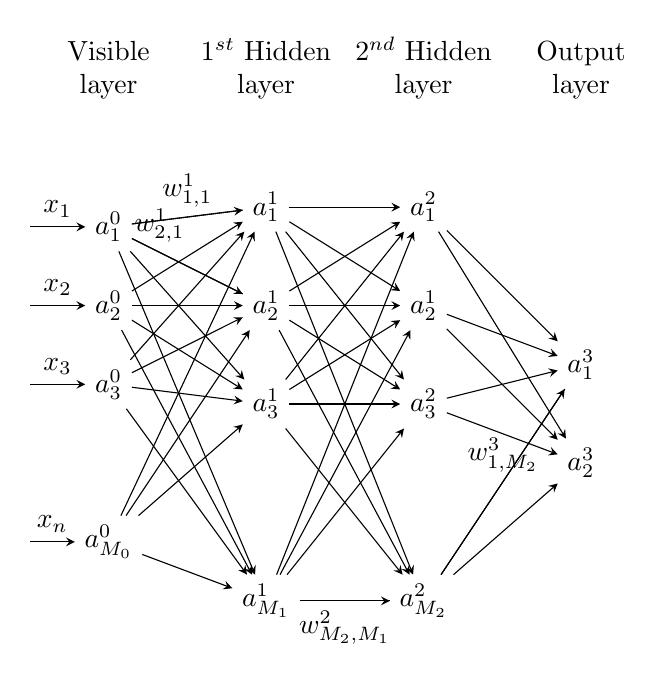
\begin{tikzpicture}[x=1cm, y=1cm, >=stealth]

\foreach \j\m/\l [count=\y] in {$a_{1}^{0}$/1,$a_{2}^0$/2,$a_{3}^0$/3,/missing,$a_{M_0}^0$/4}
  \node [every neuron/.try, neuron \m/.try] (input-\m) at (0,2.5-\y) {\j};

\foreach \j\m [count=\y] in {$a_{1}^1$/1,$a_{2}^1$/2,$a_{3}^1$/3,/missing,$a_{M_1}^1$/4}
  \node [every neuron/.try, neuron \m/.try ] (hidden1-\m) at (2,3-\y*1.25) {\j};

\foreach \j\m [count=\y] in {$a_{1}^2$/1,$a_{2}^1$/2,$a_{3}^2$/3,/missing,$a_{M_2}^2$/4}
  \node [every neuron/.try, neuron \m/.try ] (hidden2-\m) at (4,3-\y*1.25) {\j};

\foreach \j\m [count=\y] in {$a_1^3$/1,$a_2^3$/2}
  \node [every neuron/.try, neuron \m/.try ] (output-\m) at (6,1-\y*1.25) {\j};

\foreach \l [count=\i] in {1,2,3,n}
  \draw [<-] (input-\i) -- ++(-1,0)
    node [above, midway] {$x_\l$};
    
\foreach \i in {1,...,4}
  \foreach \j in {1,...,4}
    \draw [->] (input-\i) -- (hidden1-\j);


\foreach \i in {1,...,4}
  \foreach \j in {1,...,4}
    \draw [->] (hidden1-\i) -- (hidden2-\j);


\foreach \i in {1,...,4}
  \foreach \j in {1,...,2}
    \draw [->] (hidden2-\i) -- (output-\j);


\draw [-] (input-1) -- (hidden1-1)
 node [above, midway] {$w^1_{1,1}$};
 
\draw [-] (input-1) -- (hidden1-2)
 node [above, near start] {$w^1_{2,1}$}; 
 
\draw [-] (hidden1-4) -- (hidden2-4)
 node [below, midway] {$w^2_{M_2,M_1}$};

\draw [-] (hidden2-4) -- (output-1)
 node [above, midway] {$w^3_{1,M_2}$};

\foreach \l [count=\x from 0] in {Visible, $1^{st}$ Hidden, $2^{nd}$ Hidden, Output}
  \node [align=center, above] at (\x*2,3) {\l \\ layer};
\end{tikzpicture}


\end{frame}


\end{document}

